% CVPR 2026 project report using the official cvpr-org author kit.
\documentclass[10pt,twocolumn,letterpaper]{article}
\usepackage[pagenumbers]{cvpr}
\usepackage{times}
\usepackage{graphicx}
\usepackage{booktabs}
\usepackage{multirow}
\usepackage{microtype}
\usepackage{enumitem}
\usepackage{balance}
\definecolor{cvprblue}{rgb}{0.21,0.49,0.74}
\usepackage[colorlinks,allcolors=cvprblue]{hyperref}
\newcommand{\SeedMean}{76.0}
\newcommand{\SeedStd}{5.8}
\newcommand{\SeedMin}{68}
\newcommand{\SeedMax}{82}
\newcommand{\SeedPooledSuccess}{190}
\newcommand{\SeedPooledEpisodes}{250}
\newcommand{\CoverageOneDemo}{6}
\newcommand{\CoverageCleanFiveHundred}{2}
\newcommand{\CoverageAppearancePoseTwoThousand}{20}
\newcommand{\CoveragePlusCameraThreeThousand}{50}
\newcommand{\CoveragePlusCombinedFourThousand}{82}
\newcommand{\CoverageOracle}{100}
\newcommand{\CameraZerocm}{98}
\newcommand{\CameraOnecm}{94}
\newcommand{\CameraTwocm}{76}
\newcommand{\CameraThreecm}{60}
\newcommand{\CameraFourcm}{50}


\def\confName{CVPR}
\def\confYear{2026}
\title{OneVideo2Policy: A Resource-Constrained Reproduction of\\
Synthetic Robot Learning from One Human Video}
\author{Anonymous Author\\Project Report}

\begin{document}
\maketitle

\begin{abstract}
Video2Robo proposes converting one monocular human demonstration into diverse
robot training data using object tracking, 3D Gaussian Splatting (3DGS), and
kinematically coupled robot motion. We study which parts of this claim survive on
a single 6\,GB consumer GPU without physical robots. Our pipeline uses SAM~2.1
Small and CoTracker3 for perception, evaluates TripoSR and Stable Fast 3D as
lightweight reconstruction candidates, retains measured RGB-D geometry when both
learned meshes fail a frozen proportion gate, and trains a 2.61M-parameter
dual-view waypoint estimator for a measured ball-to-bowl task in robosuite.
Across five training seeds and 250 paired combined-shift rollouts, the selected
pipeline obtains \SeedMean$\pm$\SeedStd\% mean success. A cumulative coverage
ablation rises from \CoverageCleanFiveHundred\% with 500 clean frames to
\CoveragePlusCombinedFourThousand\% with 4,000 frames spanning Gaussian appearance,
robot pose, camera, and lighting variation, although the five-seed mean remains
below the frozen 80\% combined-shift gate. Correspondence-constrained motion
estimation reduces held-out image-plane error from 34.89 to 0.70 pixels, while
single-image meshes retain 33--59\% maximum secondary-dimension error. These
results support synthetic visual diversity for simulated robustness, but also
show that rendering fidelity, metric geometry, and closed-loop policy quality
must be evaluated separately. We make no physical transfer claim.
\end{abstract}

\section{Introduction}
Robot imitation learning is limited by the cost of collecting diverse
demonstrations. Video2Robo~\cite{deng2026video2robo} addresses this bottleneck by
recovering task-relevant motion from one RGB human video, editing a 3DGS scene,
and rendering robot demonstrations under object, appearance, lighting, and
viewpoint changes. Its evaluation uses six tasks, an NVIDIA L40 GPU, Diffusion
Policy~\cite{chi2023diffusion}, and physical Franka arms. This leaves a practical
question: what evidence can be reproduced on a small local machine when real
robots and high-memory accelerators are unavailable?

We answer this question through a scoped reproduction rather than a claim of
method equivalence. The running task is rigid-object placement using one HOI4D
ball-to-bowl sequence~\cite{liu2022hoi4d}. The evaluation separates four links in
the pipeline: perception, metric reconstruction, appearance generation, and
closed-loop control. This separation matters because a visually plausible mesh
may be unsafe for collision geometry, a higher-PSNR render may shift the policy
input, and low offline action error may still yield zero closed-loop success.

Our study asks three questions. \textbf{RQ1:} can small perception and
reconstruction models recover useful motion and geometry? \textbf{RQ2:} which
forms of synthetic coverage improve robustness under combined visual and camera
shift? \textbf{RQ3:} are the selected results stable across training seeds and
increasing camera displacement? Our contributions are:
\begin{itemize}[leftmargin=*,nosep]
  \item a gated, reproducible video-to-simulation pipeline that runs on 6\,GB VRAM;
  \item controlled reconstruction, tracking, Gaussian, policy, and resource measurements;
  \item five-seed paired evaluation and coverage/severity ablations; and
  \item explicit negative results for learned metric meshes and direct low-level visual policies.
\end{itemize}

\begin{figure}[t]
  \centering
  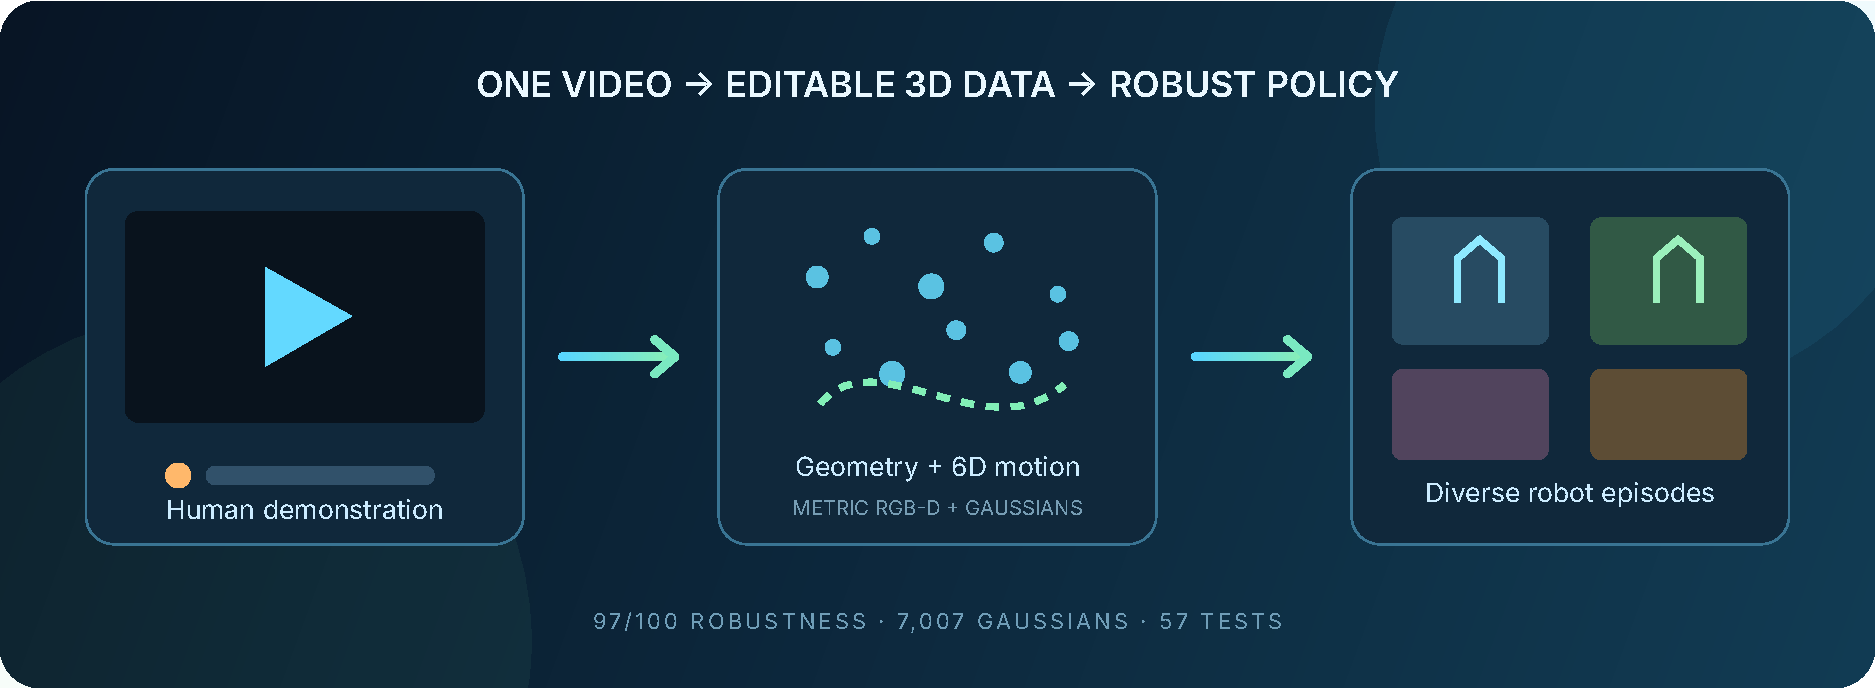
\includegraphics[width=\linewidth]{project-overview.pdf}
  \caption{Hardware-free reproduction. One human sequence supplies masks,
  tracks, metric anchors, and object-relative motion. Measured geometry drives
  physics; 3DGS supplies appearance diversity; the learned component estimates
  a visual waypoint used by a validated phase controller.}
  \label{fig:pipeline}
\end{figure}

\section{Method and Evaluation Design}
\paragraph{Perception and motion.}
We run SAM~2.1 Hiera Small~\cite{ravi2024sam2} and offline
CoTracker3~\cite{karaev2025cotracker3} over 72 frames. The source and target
retain fixed identities; tracked pixels constrain frame-to-frame pose. For an
asymmetric Record3D action-camera sequence, we compare mask centroid/area/principal
axis fitting against correspondence-constrained 2D similarity fitting. Every
third spatially sorted verified match is held out, giving 82 test
correspondences over 13 frames.

\paragraph{Geometry and appearance.}
TripoSR~\cite{tochilkin2024triposr} and SF3D~\cite{boss2024sf3d} reconstruct an
asymmetric object from one segmented RGB frame. After aligning each longest axis
to an RGB-D reference, a mesh passes only if both secondary extents are within
15\%. Failed learned meshes remain visual proposals; metric RGB-D and fitted
primitives drive robosuite~\cite{zhu2020robosuite} physics. A sparse RGB-D 3DGS
scene~\cite{kerbl2023gaussians} is tuned on one frame and tested on three held-out
views. Semantic anchors register simulator foreground to the Gaussian scene and
depth ordering handles occlusion.

\paragraph{Policy.}
The task uses a 38.32\,mm ball and a 99.12$\times$56.93\,mm bowl. The selected
policy is a 2.61M-parameter dual-view CNN that predicts the ball waypoint from
two 84$\times$84 RGB views. A phase controller performs approach, grasp,
transfer, release, and retreat. This hybrid design differs from Video2Robo's
end-to-end Diffusion Policy and is evaluated as learned visual localization plus
scripted control. Direct one-step, chunked, absolute-joint, and compact diffusion
policies are retained as negative baselines.

\paragraph{New statistical protocol.}
Five models are trained with seeds 42--46 on the same 4,000-frame dataset. Each
is evaluated on 50 identical resets with random object pose, independent
$\pm2$\,cm translations of both cameras, half lighting, and a Gaussian
background. We report mean and sample standard deviation over training seeds;
paired resets support exact McNemar comparisons. A cumulative coverage ladder
uses 1 demonstration, 500 clean frames, 2,000 frames with Gaussian/robot-pose
coverage, 3,000 frames adding camera jitter, and 4,000 frames adding joint
camera/lighting variation. A separate curve varies camera translation from 0 to
4\,cm. No physical trial is included.

\section{Results}
\subsection{Perception, geometry, and rendering}
SAM/CoTracker passes the frozen perception gate: mean mask IoU is 0.777 for the
moving source and 0.920 for the target, track survival is 91.4\% and 95.1\%, and
there are no identity swaps. Correspondences are decisive for observable
rotation: median held-out error falls by 98.0\%, from 34.89 pixels
(95\% bootstrap CI 34.25--36.11) to 0.70 (0.57--0.91).

\begin{table}[t]
\centering
\caption{Single-image reconstruction after longest-axis metric alignment. Both
learned meshes fail the 15\% secondary-extent gate.}
\label{tab:geometry}
\setlength{\tabcolsep}{3.2pt}
\resizebox{\linewidth}{!}{%
\begin{tabular}{lrrrr}
\toprule
Geometry & Extents (mm) & Max err. & Watertight & VRAM \\
\midrule
RGB-D reference & 81.9/60.6/35.4 & --- & --- & --- \\
TripoSR-128 & 81.9/69.7/14.5 & 58.9\% & yes & 1.87\,GB \\
SF3D & 81.9/68.3/23.7 & 33.1\% & no & 6.17\,GB \\
\bottomrule
\end{tabular}
}
\end{table}

Table~\ref{tab:geometry} shows that SF3D is proportionally closer but consumes
the full device and is non-watertight; TripoSR is practical for visualization but
flattens the unseen dimension. The metric path therefore uses RGB-D or
primitives. The 7,007-Gaussian scene gains 0.49\,dB mean PSNR on three held-out
views after footprint tuning. Yet the tuned render lowers downstream success
from 20/20 to 18/20, and retraining reaches 17/20. Image reconstruction quality
therefore does not provide a policy-selection metric by itself. Metric
registration yields 2.7\,mm median table-plane residual and 99.2\% depth-visible
simulator foreground.

\subsection{Closed-loop policy evidence}
Table~\ref{tab:controllers} reports architecture controls from 100 successful
robosuite demonstrations. The compact direct visual policies all fail from held-out
initializations despite low validation losses. The temporal waypoint interface
instead succeeds in 19/20 trials. This result narrows the claim: learning stable
spatial state and retaining an explicit controller works locally; it does not
reproduce Video2Robo's learned absolute-joint policy.

\begin{table}[t]
\centering
\caption{Closed-loop controls on held-out resets. Small $n$ rows are diagnostic;
the selected policy receives the larger robustness study below.}
\label{tab:controllers}
\setlength{\tabcolsep}{4pt}
\begin{tabular}{lrr}
\toprule
Policy & Success & Parameters \\
\midrule
Privileged state MLP & 8/20 & 82k \\
Phase-conditioned image BC & 0/5 & 335k \\
Dual-view action chunking & 0/5 & 640k \\
Compact diffusion & 0/5 & 944k \\
Absolute-joint chunking & 0/5 & 643k \\
Temporal visual waypoint (ours) & \textbf{19/20} & 2.61M \\
\bottomrule
\end{tabular}
\end{table}

Across the new five-seed combined-shift experiment, mean success is
\textbf{\SeedMean$\pm$\SeedStd\%}, with seed outcomes spanning
\SeedMin--\SeedMax\%. This uses \SeedPooledSuccess/\SeedPooledEpisodes successful
rollouts in total, but the seed distribution is the unit of replication. The
mean falls below the frozen 80\% combined-shift gate, revising the conclusion
drawn from the originally selected checkpoint. That checkpoint attained 20/20
nominal, 19/20 camera, 20/20 half-light, 20/20 Gaussian-background, and 18/20
combined successes; the repeated experiment shows that checkpoint selection hid
material optimization variance.

\begin{figure*}[t]
  \centering
  \begin{minipage}{0.48\textwidth}
    \centering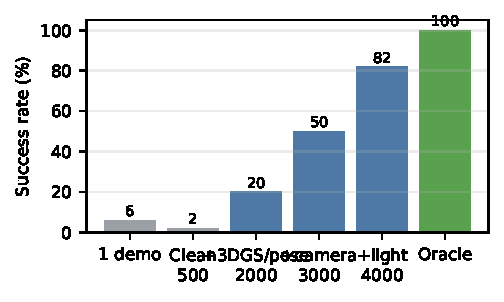
\includegraphics[width=\linewidth]{coverage-ablation.pdf}
  \end{minipage}\hfill
  \begin{minipage}{0.48\textwidth}
    \centering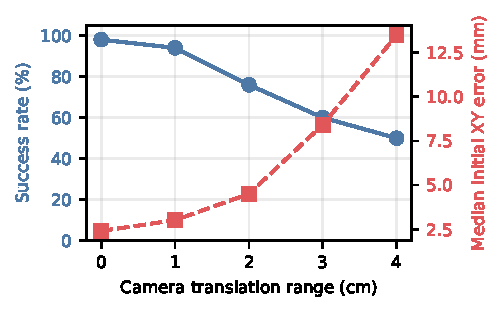
\includegraphics[width=\linewidth]{camera-severity.pdf}
  \end{minipage}
  \caption{\textbf{Left:} paired combined-shift coverage ablation. Adding the
  shift observed at test time is more important than raw frame count.
  \textbf{Right:} success and initial localization error as camera translation
  exceeds the training range. Each point uses 50 identical resets.}
  \label{fig:newexperiments}
\end{figure*}

The coverage ladder in Fig.~\ref{fig:newexperiments} rises from
\CoverageOneDemo\% (one demonstration) and \CoverageCleanFiveHundred\% (500 clean
frames) to \CoverageAppearancePoseTwoThousand\% after appearance and robot-pose
coverage. Adding camera data produces \CoveragePlusCameraThreeThousand\%, while explicit
combined-shift examples reach \CoveragePlusCombinedFourThousand\%; exact simulator
geometry gives the \CoverageOracle\% controller ceiling. This is evidence for
coverage alignment rather than a generic ``more data'' effect because the stages
change both sample count and variation type. The camera curve remains at
\CameraZerocm--\CameraTwocm\% through the trained 0--2\,cm range, then reaches
\CameraThreecm\% and \CameraFourcm\% at 3 and 4\,cm, locating an empirical
viewpoint boundary rather than reporting one arbitrary perturbation.

\subsection{Efficiency}
The full local stack fits a GTX 1660 Ti. TripoSR peaks at 1.87\,GB; SF3D peaks at
6.17\,GB. Depth Anything V2 Small peaks at 415\,MiB with 0.159\,s median
inference. Rendering the final 4,000-frame localization set is the main local
data cost; training the 2.61M-parameter policy takes 55.4\,s. One complete
depth-ordered Gaussian robot demonstration contains 353 synchronized dual-view
samples. These measurements complement Video2Robo's L40 results and expose the
accuracy lost when choosing small feed-forward geometry models.

\subsection{Statistical contrasts and failure modes}
Because every coverage variant sees the same 50 resets, we compare binary
outcomes with two-sided exact McNemar tests. The 4,000-frame model beats the
3,000-frame camera model on 16 discordant episodes with no reverse discordance
($p=3.05\times10^{-5}$). Its advantage over the 2,000-frame appearance/pose
model is also decisive (32 gains and one loss, $p<10^{-8}$). These paired tests
do not prove that frame count is causal: the ladder intentionally adds examples
from a new shift at each stage. They do show that the observed gains are not a
consequence of different reset difficulty.

Failure traces connect success to perception. Under the combined shift, the
full model's 41 successful episodes have 4.47\,mm median initial XY error; its
nine failures have 11.90\,mm. Eight of those failures terminate during the
gripper-close phase, consistent with a missed grasp, while one reaches the final
phase without satisfying placement. At 4\,cm camera shift, successful and failed
episodes separate further (8.12 versus 23.40\,mm median error). Fourteen of 25
failures terminate at gripper close and nine fail during approach. The controller
ceiling remains 50/50 under the combined condition, so the dominant measured
bottleneck is visual localization rather than task physics.

The five-seed experiment exposes a second failure mode: model selection variance.
All models use the same architecture, dataset, optimizer, and paired test resets,
yet combined success spans 68--82\%. Their median XY errors are much less variable
(4.94--5.95\,mm), indicating that a few tail predictions determine many grasp
outcomes. Reporting only the best checkpoint therefore overstates reliability.
The 95\% $t$ interval for mean seed success is 68.8--83.2\%; it crosses the 80\%
gate but does not establish a pass. More seeds or a tail-aware training objective
would be needed to narrow this uncertainty.

\section{Relationship to Video2Robo}
Table~\ref{tab:scope} states the intended comparison. Video2Robo evaluates six
tasks and trains an absolute-joint Diffusion Policy from photorealistic robot
videos. It reports 63.83\% mean simulated success under multiple variation types,
compared with 11.67--44.67\% for its MimicGen/SkillGen controls, and performs
physical Franka trials~\cite{mandlekar2023mimicgen,garrett2024skillgen}. Our
higher task-specific percentages are not directly
comparable: the task, policy interface, geometry source, and evaluation
distribution differ. The useful reproduction question is whether the same
qualitative factors---temporal tracking and frame-level scene diversity---remain
important under a severe hardware budget. The ablations answer yes, while the
seed study adds a robustness qualification absent from a single selected run.

\begin{table}[t]
\centering
\caption{Scope comparison. ``Ours'' is designed to diagnose a small-machine
reproduction and cannot support Video2Robo's physical-transfer claim.}
\label{tab:scope}
\setlength{\tabcolsep}{3.5pt}
\resizebox{\linewidth}{!}{%
\begin{tabular}{lll}
\toprule
Dimension & Video2Robo & Ours \\
\midrule
Tasks & 6 rigid tasks & 1 rigid Place task \\
Video input & Monocular RGB & RGB + RGB-D metric anchors \\
Geometry & learned scale/3DGS & measured primitives \\
Policy & Diffusion, joint targets & waypoint + phase control \\
Training GPU & NVIDIA L40 & GTX 1660 Ti, 6\,GB \\
Simulation & pose + multi-shift & five controlled conditions \\
Physical robot & Franka, two cameras & out of scope \\
Repeated seeds & not reported & 5 training seeds \\
\bottomrule
\end{tabular}
}
\end{table}

The comparison also clarifies what Gaussian splatting contributes here. In
Video2Robo, 3DGS represents editable task objects and the scene, supporting
view-consistent robot data. In our retained policy dataset, simulator foreground
is composited over an animated Gaussian background; metric registration is
demonstrated separately but is not used to train the selected checkpoint. The
experiment therefore tests Gaussian appearance coverage, not a complete
3DGS-based robotization pipeline. This narrower interpretation is necessary for
an accurate report.

\section{Discussion and Limitations}
Three findings follow. \textbf{First, temporal correspondences are necessary.}
Mask-only pose fitting is visually plausible yet inaccurate on an asymmetric
object. \textbf{Second, visual reconstruction and metric reconstruction are
different objectives.} Neither learned mesh supports the frozen collision gate,
and higher held-out PSNR does not select the best controller input.
\textbf{Third, data must cover the deployment shift, but coverage is not
sufficient for seed-stable robustness.} Gaussian appearance alone does not
repair camera geometry; explicit camera and low-light examples produce the
largest combined-shift gain, while the five-seed mean still misses the 80\% gate.

The study has clear boundaries. It contains one manipulation task, uses RGB-D
scale and primitives rather than a monocular-only geometry estimate, composites
Gaussian appearance around simulator foreground, and delegates phase execution
to a scripted controller. The five training seeds share one generated dataset,
so they measure optimization variability rather than source-video variability.
No robot hardware is available; physical success and sim-to-real transfer remain
unevaluated. Compared with Video2Robo's six-task study and physical Franka trials,
this report establishes a resource-constrained simulation result only.

\section{Reproducibility and Future Work}
The experiment runner freezes the 4,000-frame dataset, five training seeds, one
paired reset seed, and 50 episodes per checkpoint. It resumes only from a report
whose episode count matches the requested protocol, then regenerates JSON
aggregates, LaTeX macros, and both plots. Raw observations, checkpoints, and
episode traces stay outside version control because of their size; the committed
manifest records their paths and the aggregate contains Wilson intervals, the
seed distribution, and paired tests. This design makes the PDF a derived artifact
of the same measurements rather than a manually transcribed summary.

Three extensions would materially change the evidence. First, repeat the entire
pipeline on at least Place, Stack, and Sweep. These tasks add vertical placement
and sustained contact, testing whether the waypoint interface is specific to a
spherical pick-and-place task. Each task should use an independent source video,
five training seeds, and the same pose-only and multi-shift split. Second, compare
the hybrid controller with an end-to-end action policy under an equal dataset and
action horizon. Our compact diffusion negative result is diagnostic, but a tuned
Diffusion Policy baseline is required before attributing the gap to policy class.
Third, train from the metrically registered depth-ordered Gaussian sequence rather
than appearance compositing. That would test the contribution of view-consistent
3DGS robotization and make the comparison to Video2Robo substantially closer.

The current camera curve also suggests a targeted algorithmic experiment. Errors
grow smoothly from 2.42\,mm at zero camera shift to 13.46\,mm at 4\,cm, while
success falls from 98\% to 50\%. Training could sample a wider camera volume, but
that may trade nominal precision for coverage. A factorial study should therefore
cross camera range with calibration-aware inputs and report the whole severity
curve, not tune on the 4\,cm endpoint. Tail-aware objectives or ensembles may also
reduce seed variance because median localization changes little across seeds while
rare outliers determine grasp failure.

Finally, the monocular premise should be tested rather than assumed. A multi-object
benchmark can compare learned depth/mesh scale, one manual dimension, RGB-D, and
ground-truth simulator geometry using dimension error, ADD-S or BOP recall,
collision validity, and downstream success. The present results predict that
single-image mesh appearance will correlate weakly with metric fitness. Confirming
that prediction across symmetric, thin, low-texture, and partly occluded objects
would turn a task-specific engineering observation into a broader empirical result.

\section{Conclusion}
OneVideo2Policy reproduces a useful subset of the one-video synthetic-data
pipeline on 6\,GB VRAM. The strongest evidence is not a claim of end-to-end
Video2Robo equivalence, but a set of measured boundaries: correspondence tracking
stabilizes motion, lightweight single-image meshes do not provide metric physics,
and matched 3D appearance/camera/lighting coverage improves a compact learned
waypoint policy but does not produce seed-stable combined-shift robustness.
Broader tasks, source videos, and more stable training are the next hardware-free
steps; physical validation requires a different study.

\balance
{\small
\bibliographystyle{ieeenat_fullname}
\bibliography{references}
}

\end{document}
